\documentclass[a4paper,8pt]{extarticle}
\usepackage{graphicx}
\usepackage{geometry}
\usepackage[utf8]{inputenc}
\usepackage{amsmath}
\usepackage{amssymb}
\usepackage{hyperref}
\usepackage{tikz}
\usetikzlibrary{shapes,arrows,chains}
\usetikzlibrary[calc]

\title{The Evolution of Conformist Transmission}
\author{Ciaran Neely \& Yuyang Wei}
\date{April 2022}

\begin{document}

\begin{center}
    $ $
    \vfill
    \Huge{\textbf{The Evolution of Conformist Transmission\\}}
    \vspace{10pt}
    \LARGE{Ciaran Neely \& Yuyang Wei}
    \vfill
\end{center}

\thispagestyle{empty}
\newpage
\tableofcontents
\thispagestyle{empty}
\newpage
\pagenumbering{arabic}
\section{Abstract}
In this paper we examine a memetic transmission pattern known as conformist transmission, wherein individuals preferentially adopt behaviours which occur most frequently in the population. The existence of such transmission patterns may be important in explaining the observed lack of genetic diversity within humans compared to other cosmopolitan species. We do this using a model originally developed by Boyd \& Richerson (1985) and later expanded upon by Henrich & Boyd (1998). We show that genetic alleles causing a preference toward social learning with a bias toward conformity will remain stable within a population in a wide variety of situations, even when made to compete with strategies such as individual learning. We then extend this model by allowing individuals' learning style to be not only genetically determined, but itself a learned trait subject to some of the same forces that other behaviours are chosen by. We determine that this does not qualitatively change the behaviour of the system.
\section{Introduction}
Stable human populations can be found across the globe in a wide variety of environmental conditions. Based on the patterns we see in other species, it should therefore be safe to assume that humans possess a high degree of genetic diversity. However, actual research on this subject has shown this to be false. Humans in fact possess an exceptionally low amount of genetic diversity for what we should expect from a species in our situation (Henrich 2016). This fact posses a problem in our understanding of human evolutionary biology. What is it that makes us so special? It has been argued by some that humans are simply more intelligent than other species on an individual level, and that our success can be entirely accounted for by our ability to think critically and make rational choices (Boyd \& Richerson, 1985). This view has been challenged both by Blackmore (1999), and rather extensively by Henrich (2014, 2016). The former has questioned the short-term genetic utility of developing such an organ as the human brain, given the immense costs associated with it. And many case studies of lost European explorers throughout history have shown that otherwise intelligent humans can easily starve to death in regions where local populations of their own species have been thriving for millennia (Henrich 2014, 2016). For one of many examples provided by Henrich (2014, 2016), consider the famous case of Burke \& Wills' who spent their final days stranded in the Australian outback in the aftermath of a failed expedition. If we accept the hypothesis the human ability to adapt to new environmental conditions is simply a result of individual intelligence within a genetically homogeneous species, then why is it that Burke \& Wills could not figure out those survival skills that the Yandruwandha tribe had figured out several thousand years prior? We do not wish to claim that individual intelligence plays \emph{no} part in human adaptability, just that it is not give a full picture. The reality is that the solutions available to overcome the problems our hunter-gatherer ancestors have faced are often not at all obvious. And at least in the modern hunter-gatherer populations which have been studied by anthropologists, individuals frequently engage in highly adaptive behaviours without being able to explain \emph{why} they have chosen to behave in the way they do (Henrich, 2014). The model we examine in this paper will however provide a role for individual learning, which takes into account the non-obvious nature of environmental cues.
\\\\
Both Blackmore (1999) and Henrich (2014, 2016), as well as many in the field of anthropology (Henrich \& Boyd, 1998) claim that the central aspect that makes our species so exceptional is culture. Along with orcas (Henrich, 2014) and certain species of songbird (Dawkins, 2006), humans are  the few species on this planet that may rightfully be called a ``cultural species"; and even within this small subset we are in fact quite exceptional, to the point that human behaviour cannot always be well-understood with the tools typically applied to most other organisms (Boyd \& Richerson, 1985). Analogies have been made by Dawkins (1982, 2006) and Blackmore (1999) between ``memes" (the units of cultural transmission) and biological systems such as genes and viruses. This is a good starting point, and with it we may propose the following null hypothesis: Perhaps genetic and memetic transmission are in most cases functionally identical, and for the purposes of modelling population dynamics, we can simply treat memes as though they occupy some imaginary $24^{\text{th}}$ ``chromosome" where information is stored not in the form of nucleotide base-pairs, but using some type of analogous mental process, the precise nature of which can be left as a problem for the psychophysiologists to work out. This hypothesis could account for all the ``genetic" diversity we expect to see within our species, and though it would not address \emph{all} our sociobiological peculiarities, it would address the central question that we have posed in the introduction to this paper. However analysis done by Cavalli-Sforza \& Feldman (1983) shows that in simple models of this kind, cultural adaptations almost always die out if a similar adaptation is achievable through genetic means, since genetic adaptation can reasonably be assumed to have an edge in terms of efficiency. Furthermore, leaning more into the ``virus" analogy and allowing memes to be spread laterally and/or obliquely throughout the population was shown to have little to no qualitative effect on the behaviour of the system. It therefore may be necessary to consider the potential transmission patterns available to memes which do not have analogues in biology. We will examine one such pattern. 

\section{Conformist Transmission}
Generally in biological systems, traits (including symptoms of disease) are transmitted through a mechanism known as ``frequency-independent" transmission. Under this paradigm, the effect of transmission (barring all other forces) is to preserve relative frequencies of traits within the population. For instance, consider some population infected with two mutually exclusive but functionally identical strains of a given virus, such that $60\%$ of the population are infected with strain-$A$, and $40\%$ are infected with strain-$B$. Using a simple two-strain model (Brauer et al. 2008), it can be shown that if we introduce a new susceptible individual into the population, then, given that they become infected, there is a $60\%$ chance that the infection is with strain-$A$ and a $40\%$ chance the infection is with strain-$B$. Hence, on average, the addition of new susceptible individuals into the population has no effect on the relative frequencies of the two competing strains. Any change in the relative frequency over time therefore must be a result of differences in the local properties of the two strains, (i.e. infection rate, recovery rate, etc.), and not on their frequency within the population. Similar dynamics occur when considering two competing alleles in a population that is in Hardy-Weinberg equilibrium (Herron \& Freeman, 2014). 
\\\\
In this paper based off the work of Henrich \& Boyd (1998), and Boyd \& Richerson (1985), we investigate a transmission pattern known as ``conformist transmission". Under this paradigm, naïve individuals are disproportionately more likely to adopt memes which occur more frequently in the population. For instance, if $60\%$ of individuals within a population express behaviour $A$ and $40\%$ express behaviour $B$, then a naïve individual may have a $75\%$ chance of adopting  $A$, and only a $25\%$ chance of adopting $B$. As a result, unless other forces are at play, the frequency of behaviour $A$ will continually increase over time as the population gets recycled.
\\\\
Since cultural systems ostensibly evolved out of biological systems, it is reasonable to assume that conformist transmission evolved out of a landscape initially governed by frequency-independent transmission. This provides a line of support for advent of conformist transmission, since under frequency-independent models in a stable environment, selection will result in the most adaptive trait present within a population eventually becoming the most common (Boyd \& Richerson, 1985). However we cannot know without further analysis whether the frequency of a given trait will continue to be a useful indicator of its adaptiveness as conformists begin to dominate the population.
\\\\
We will also account for the effect of unstable environments, which has been suggested as a potential pitfall for conformist transmission models, since once-adaptive behaviours may become ``locked in" even after conditions change such a way that makes them maladaptive (Henrich \& Boyd, 1998). For instance, a population of conformists may learn that a particular species of mushroom is safe to eat. Individuals who regularly eat them will then face higher fitness in the form of better food security than those who refuse, eventually causing that behaviour to dominate the population. This however, then may cause that species of mushroom to evolve defenses against its predators in the form of some acute toxicity. Conformists may however may not be deterred, even in the face of debilitating illness, creating a vicious cycle wherein an entire population poisons themselves simply because it is what everyone else in the population is doing. Or to use a more concrete (and perhaps to some, familiar) example, a population of conformists living in certain regions of the United States may find a useful cultural adaptation for differentiating between the (dangerous) eastern coral snake and the (harmless) scarlet kingsnake in the form of a rhyme: ``Red touches black, venom lack. Red touches yellow, kill a fellow". However, this rhyme may persist even as the population migrates southward into the territory of the aquatic coralsnake, which is highly venomous \emph{despite} its red-touches-black colouration (Valen, 2020). 
\section{Design}
A diagram of the model is provided in Figure \ref{fig:4.1}. Simulations can be defined by the following global parameters:
\begin{enumerate}
    \item $m\in[0,1]$ is the rate of migration between sub-populations.
    \item For each $i\in \mathcal I$, $W_{iB}\in\{1.00, 1.01\}$ is a measure of the adaptiveness of behaviour $B$ within environment $i$. When $W_{iB}=1.01$, we consider behaviour $B$ to be ``adaptive" within the environment $i$. When $W_{iB}=1.00$ we consider behaviour $B$ to be maladaptive in environment $i$.
    \item $\epsilon\in[.5,1]$ measures the stability of the environment, i.e. the probability that a given sub-population will experience the same environmental condition in the next generation. 
    \item $\rho\in[.5,1)$ represents the accuracy of environmental cues. A $\rho$-value close to 1 implies that which behaviour is adaptive is very obvious to individuals in the simulation. Examples of $\rho\approx 1$ behaviours are those which are comically straightforward, such as walking off a cliff or generally eating food. Even without any background in the nuances of evolutionary biology, it does not take a genius to figure out which of the aforementioned behaviours are adaptive and which are maladaptive compared to their alternatives (I'll give you a hint: there is one of each). On the other hand, a value of $\rho=.5$ implies that the environment provides no information as to weather a behaviour is adaptive, and hence individual learning amounts to a coin flip. For instance, a real-world example of a $\rho\approx.5$ behaviour might be the practice of adding ash from burnt seashells into cornmeal during its preparation. This was practiced by populations in the Americas, and prevented them from contracting pellagra despite their corn-rich diet. When corn was later brought over to the Old World between the $16^{\text{th}}$ and $18^{\text{th}}$ centuries, pellagra became a widespread issue in many European communities. Yet it was not until the $20^{\text{th}}$ century that European scientists were able to determine the cause of the disease (Henrich, 2014). It is therefore highly unlikely that any one individual in a population would be able to have \emph{justified true believe} about this connection and derive the practice simply by virtue of their own life experience.
\end{enumerate}
For all $B\in\{E,\lnot E\}$, $i\in\mathcal I$, $\lambda\in\mathcal J$, $\theta\in\mathcal K$, let $u_{iB\lambda\theta}(t)$ be the rate at which individuals experience both behaviour $B$ and genotype $(\lambda,\theta)$ within sub-population $i$, as a function of time $t$. Each integer value of $t$ represents one generation. Generation $t=0$ gives birth to generation $t=1$, who gives birth to generation $t=2$, and so on. On top of this, we use non-integer intermediate values of $t$ to represent the 4 life stages that individuals go through within a single generation. The four stages can be modelled with the following four difference equations

\tikzstyle{block} = [rectangle, draw, text centered]
\tikzstyle{arrow} = [draw, -latex']

\begin{figure}
    \centering
    \begin{tikzpicture}
        %\node[block] at (0,8) (gen00) {Gen 0.0};
        %\node[block] at (4,8) (gen01) {Gen 0.1};
        %\node[block] at (8,8) (gen02) {Gen 0.2};
        \node[block] at (12,8) (gen03) {Initial State};
        
        \node[block] at (0,4) (gen10) {Gen 1.0};
        \node[block] at (4,4) (gen11) {Gen 1.1};
        \node[block] at (8,4) (gen12) {Gen 1.2};
        \node[block] at (12,4) (gen13) {Gen 1.3};
        \node[scale=2] at (1,0) (ellipsis) {$\cdots$};
        
        %\path[arrow] (gen00) -- node [text width=2.5cm,midway,above,align=center] {Learning} (gen01);
        %\path[arrow] (gen01) -- node [text width=2.5cm,midway,above,align=center] {Migration} (gen02);
        %\path[arrow] (gen02) -- node [text width=2.5cm,midway,above,align=center] {Selection} (gen03);
        
        \draw (gen03) -- (13.5,8) -- (13.5,6) -- (-1.5,6) -- (-1.5,4);
        \draw[-stealth] (-1.5,4) -- (gen10);
        \path (13.5,6) -- node [text width=2.5cm,midway,above,align=center] { Transmission} (-1.5,6) ;
        
        \draw (gen13) -- (13.5,4) -- (13.5,2) -- (-1.5,2) -- (-1.5,0);
        \draw[-stealth] (-1.5,0) -- (0,0);
        \path (13.5,2) -- node [text width=2.5cm,midway,above,align=center] { Transmission} (-1.5,2) ;
        
        
        \path[arrow] (gen10) -- node [text width=2.5cm,midway,above,align=center] {Ind. Learning} (gen11);
        \path[arrow] (gen11) -- node [text width=2.5cm,midway,above,align=center] {Migration} (gen12);
        \path[arrow] (gen12) -- node [text width=2.5cm,midway,above,align=center] {Selection} (gen13);
    \end{tikzpicture}
    \caption{A diagram summarizing the model originally developed by Boyd \& Richerson (1985) and later expanded upon by Henrich \& Boyd (1998) showing the life stages of individuals within the population. We imagine that the population is split evenly between some set $\mathcal I$ of sub-populations. We will also assume that each sub-population is sufficiently large so as to negate the unpredictable effects of random sampling. Each individual in the population possesses some genotype \mbox{$(\lambda,\theta)$} drawn from the set of available genotypes $\mathcal J \times \mathcal K$. Each individual's genotype affects how they go about choosing between two available mutually exclusive behaviours, $B=E$ and $B=\lnot E$ (for instance, eating or not eating a particular species of mushroom). Each sub-population may face different environmental conditions. For example, one behaviour (i.e. eating the mushrooms) may be adaptive in sub-population 1, whereas in sub-population 2 the alternative behaviour (i.e. refusing to eat the mushrooms) may be adaptive. We will imagine that this all happens in a series of life stages: First, in the transmission stage, individuals inherit both genes and memes from the previous generation. Then in the Individual Learning stage, individuals faces some life experience which may cause them to question what they have learned socially. For instance, an individual may eat a particular species of mushroom and get sick soon afterwards. This could be a sign that the mushroom is poisonous, or simply an unfortunate coincidence. Then in the Migration stage individuals have the opportunity to migrate into a new sub-population where conditions may or may not be different. And then natural selection takes effect in each sub-population, favouring individuals with one of the two behaviours. From here, we once again return to the Transmission stage as Generation 2.0 is born from Generation 1.3, and the cycle repeats. } 
    \label{fig:4.1}
\end{figure}


\begin{align}
    %%%%%%%%%%%%%%
    % EQUATION 1 %
    %%%%%%%%%%%%%%
    u_{iB\lambda\theta}(t+.0)
    &=\underset{\text{(Baseline Frequency)}}{\underbrace{u_{iB\lambda\theta}((t-1)+.3)}_{\text{Unbiased Transmission}}}
    +\underbrace{
        D_\theta
        \cdot [q_{iB}-q_{(\lnot B)i}]
        \cdot q_{iB}
        \cdot q_{(\lnot B)i}
        \cdot u_{iB\lambda\theta}((t-1)+.3)}_{\text{Conformist Transmission}
    }
    \label{mod:1}
    \\
    \nonumber
    \\
    %%%%%%%%%%%%%%
    % EQUATION 2 %
    %%%%%%%%%%%%%%
    u_{iB\lambda\theta}(t+.1)
    &=
    \underbrace{u_{iB\lambda\theta}(t+.0)}_{\text{Baseline Frequency}}
    -\ \ 
    \underbrace{
        p_{(\lnot B)i\lambda}
        \cdot u_{iB\lambda\theta}(t+.0)
    }
    _{\text{Rate of Rejection of $B$}}
    +\ \ 
    \underbrace{
        p_{iB\lambda}
        \cdot u_{i(\lnot B)\lambda\theta}(t+.0)
    }
    _{\text{Rate of Adoption of $B$}}
    \label{mod:2}
    \\
    \nonumber
    \\
    %%%%%%%%%%%%%%
    % EQUATION 3 %
    %%%%%%%%%%%%%%
    u_{iB\lambda\theta}(t+.2)
    &=
    \underbrace{
        u_{iB\lambda\theta}(t+.1)
    }
    _{\text{Baseline Frequency}}
    -\ \ 
    \underbrace{
        m
        \cdot u_{iB\lambda\theta}(t+.1)
    }
    _{\text{Migration Out}}
    \ + \ 
    \underbrace{
        m
        \cdot\bar u_{B\lambda\theta}
    }
    _{\text{Migration In}}
    \label{mod:3}
    \\
    \nonumber
    \\
    %%%%%%%%%%%%%%
    % EQUATION 4 %
    %%%%%%%%%%%%%%
    u_{iB\lambda\theta}(t+.3)
    &=\frac{
        W_{Bi}
        \cdot u_{iB\lambda\theta}(t+.2)
    }{
        \overline W
    }
    \label{mod:4}
\end{align}
Equation (\ref {mod:1}), models how individuals in the population learn socially from those in the final stage of the previous generation. The $\mathcal K$-component of each individual's genotype codes for some phenotype in the form of a coefficient $D_\theta\in[0,1]$ which scales the conformist effect in this process. How we choose to represent the elements of $\mathcal K$ and define their respective $D$-values is arbitrary. All we care about is that there is a healthy amount of variation throughout the population for natural selection to work on. Hence we can keep things simple by letting \mbox{$\mathcal K=\{0,1,...,20\}$} and letting $D_\theta=\theta/20$ for all $\theta\in\mathcal K$.
\\\\
The effect of conformist transmission is also dependent on $q_{iB}$, that is, the rate at which behaviour $B$ is expressed in population $i$. More formally:
\[
    q_{iB}=
    \frac{
        \displaystyle\sum_{(\lambda,\theta)\in\mathcal J\times \mathcal K} \ u_{iB\lambda\theta}
    }{
        \displaystyle\sum_{(\lambda,\theta)\in\mathcal J\times \mathcal K} \  \Big[u_{iB\lambda\theta}+u_{i(\lnot B)\lambda\theta}\Big]
    }
\]
$q_{Bi}$ may take any real value between 0 and 1, and has the property that \mbox{$q_{Bi}+q_{(\lnot B)i}=1$}. Notice that when $B$ is more prevalent than $\lnot B$ (i.e. \mbox{$q_{Bi}>0.5>q_{(\lnot B)i}$}), the conformist effect becomes positive, causing conformists (those characterized by $D_\theta>0$) to preferentially adopt $B$ at a rate higher than its baseline frequency in the population. The inverse can be said in cases where $B$ is less prevalent than $\lnot B$. Also notice that when $q_{Bi}=1$ (i.e. when the entire sub-population already exhibits behaviour $B$), the \emph{Conformist Transmission} term will become zero, lest the model predict frequencies greater than $100\%$.
\\\\
Equation ($\ref{mod:2}$) models the effect of individuals learning from their environment. Individuals who originally learned behaviour $B$ from their peers may choose to reject it based on some personal experience. Naturally, such individuals are subtracted from the count. Similarly, individuals who original learned behaviour $\lnot B$ may choose to adopt $B$. Such individuals are added to the count. We assume that this personal experience comes in the form of cue, hinting with some level of salience, toward which behaviour is most adaptive in the environment of sub-population $i$. We assume that the salience of the cue, $X$, is normally distributed with some arbitrary standard deviation $\sigma$, around some mean $\mu$ such that $P(X\le 0)=\rho$. Using pivotal quantities of the normal distribution, we can determine that $\mu$ is the unique value such that $P(Z\le -\mu/\sigma)$ where $Z\sim G(0,1)$, and can be done in \texttt R using the \texttt {qnorm} command.
\\\\
The $\mathcal J$-component of each individual's genotype then codes for for some phenotype in the form of a threshold $H_\lambda\in[0,\infty)$, which determines how salient this cue must be in order to warrant a change in behaviour. $p_{iB\lambda}$ is the probability that an individual with a genotype characterized by $\lambda\in\mathcal J$ chooses to adopt behaviour $B$ through personal experience, and can be defined as follows:
\[
    p_{iB\lambda}=\left\{\begin{array}{ll}
         P(X\ge H_\lambda\sigma)& \text{if \quad $W_{iB}\ge W_{i(\lnot B)}$} \\\\
         P(X\le-H_\lambda\sigma)& \text{otherwise}
    \end{array}\right.
\]
Notice that $p_{iB\lambda}$ does not depend of the value we choose for $\sigma$. Thus an obvious choice is to use the simplest definition $\sigma=1$.
\\\\
Similar to how it was in Equation ($\ref{mod:1}$) with $\mathcal K$, the way we represent the relationship between elements of $\mathcal J$ and their associated $H$-values is not important so long as there is sufficient variation in the population, and we can hence define a similar linear relationship. This posses a problem however, since $H_\lambda$ can be arbitrarily large. Henrich \& Boyd (1998) solve this however by simply limiting $H_\lambda$ to a maximum value of 3.2. This can be justified by the fact that a normally distributed random variable will almost never exceed 3.2 standard deviations above or below its mean.
\\\\
Equation ($\ref{mod:3}$) models the effect of migration between sub-populations. $\bar u_{B\lambda\theta}$ is the average frequency of $B\lambda\theta$-profile within the entire population. More formally
\[
    \bar u_{B\lambda\theta}=\frac 1 {|\mathcal I|}\sum_{i\in \mathcal I} u_{iB\lambda\theta}
\]
Finally, Equation ($\ref{mod:4}$) models the effect of natural selection on the population. This is dependent on the value $\overline W$, which is the average fitness within the population as a whole. More formally
\[
    \overline W =
    \sum_{i\in \mathcal I}\ 
    \sum_{(\lambda,\theta)\in\mathcal J\times\mathcal K}\ 
    \Big[
        W_{iB}u_{iB\lambda\theta}
        +
        W_{i(\lnot B)}u_{i(\lnot B)\lambda\theta}
    \Big]
\]
Finally, after each generation has matured, before beginning the next generation, we give each environment in $\mathcal I$ a $100(1-\epsilon) \%$ chance of swapping which behaviour is favored, i.e. if $W_{iB}=1.00$, then we set $W_{iB}=1.01$ and vice versa.


\section{Implementation of the Model}

In the implementation, R studio is used as the main tool to complete the simulation. First of all, in order to store every value of $u_{iB\lambda\theta}$, a multidimensional matrix was constructed, with number of dimensions same as the number of different variables.
\\
\\
Then, with such matrix established, we could simulate the model by updating each value in each grid. Note that each $u_{iB\lambda\theta}(t)$ value is calculated based on the previous value: for instance, let t, the number of generations, be ranged from 0 to 20, then in the model, $u_{iB\lambda\theta}(t)$ is calculated by $u_{iB\lambda\theta}(t - 1 + 0.3)$, i.e. the final result after migration and selection in the last generation; $u_{iB\lambda\theta}(t + 0.1)$ is calculated based on $u_{iB\lambda\theta}(t)$: the value after learning process needs to be based on the initial value in the same generation; $u_{iB\lambda\theta}(t + 0.2)$ is calculated based on $u_{iB\lambda\theta}(t + 0.1)$, and $u_{iB\lambda\theta}(t + 0.3)$ is calculated based on $u_{iB\lambda\theta}(t + 0.2)$. 
\\
\\
Note that in order to start the simulation, except for setting up a range of fixed global parameters like $m$, $i$, $\epsilon$ and $\rho$, an initial value of $u_{iB\lambda\theta}$ is required, which is the term $u_{iB\lambda\theta}(0.3)$; then the rest can be calculated accordingly.
\\
\\
In the code for modelling, a dynamic planning structure is used: the multidimensional matrix is updated through a nested loop, where all possible values for each variable are looped over and included as a part of the calculation. In details, over each loop, some parameters that are fixed in the local scope like $q$, $p$, $\bar{W}$ and $\bar{u_{B\lambda\delta}}$ are calculated first; then, with all parameters available, the value of $u_{iB\lambda\theta}$ can be calculated and updated in the matrix. By so, in the end all grids in the matrix are updated; with all values are stored in the matrix, values of $u_{iB\lambda\theta}(t + 0.3)$, i.e. the final result of selection in each generation can be easily extracted, and the study of the change of $u$ values can be conducted.
\\
\\
The initial values are given:
\begin{center}
\begin{tabular}{||c|c|c|c|c|c|c|c|c|c|c|c|c|c|c|c|c|c|c|c|c||} 
 \hline
  Subpopulation: &1&2&3&4&5&6&7&8&9&10 \\ [0.5ex] 
 \hline\hline
 B & 1&0.95&0.9&0.85&0.8&0.75&0.7&0.65&0.6&0.55\\ 
 \hline
 not B &0&0.05&0.1&0.15&0.2&0.25&0.3&0.35&0.4&0.45\\
 \hline
\end{tabular}
\end{center}

\begin{center}
\begin{tabular}{||c|c|c|c|c|c|c|c|c|c|c|c|c|c|c|c|c|c|c|c|c||} 
 \hline
  Subpopulation: &11&12&13&14&15&16&17&18&19&20 \\ [0.5ex] 
 \hline\hline
 B &0&0.05&0.1&0.15&0.2&0.25&0.3&0.35&0.4&0.45\\ 
 \hline
 not B & 1&0.95&0.9&0.85&0.8&0.75&0.7&0.65&0.6&0.55\\
 \hline
\end{tabular}
\end{center}
\\
where the initial values are shown as proportions. For example, in subpopulation 2 there are 95\% people who favor behavior B and 5\% people who favor behavior B; thus, we say that in this group behavior B is favored.

\section{Results}
To simulate the model, some general assumptions are required. First, a simulation over 20 generations should be plenty to observe any potential trends of migration and selection: let the number of generations be 20, starting with generation 0. We divide the population into 20 subpopulation to include diversity, and the initial value in each subgroup is different from each other. Moreover, we add an assumption that subgroups from 1 to 10 favor behavior B and subgroups from 11 to 20 favor behavior not B; thus, the two sets of subgroups would have different W values (for the subgroups who favor behavior B, B certainly is more adaptive over behavior not B and thus has $W_{iB} = 1.01$ and $W_{i(\lnot{B})} = 1.00$; vice versa), and subpopulations that favor behavior B would have initial value $u_{iB\lambda\theta}$ greater than $u_{i(\lnot B)\lambda\theta}$ and vice versa.
\\
\\
With basic parameters defined, we also need to define the global parameters that are crucial to the model. These are the parameters that may change from scenes to scenes, and are the core factors whose influence on the results is what we wish to study. For one, we need to assume the value of the migration rate, $m$. In this case, we  assume the migration rate is low: $m = 0.3$, so that only a small proportion of each sub-population will ends up migrating to another sub-population. Except that, we assume that the environment is relatively stable: we set $\epsilon = 0.75$, and assume that the accuracy of environment cues is relatively high: set $\rho = 0.8$. However, since neither $\epsilon$ nor $\rho$ appears in the model, we can simply ignore them and focus on the impact of the migration rate, $m$.
\\
\\
First, we examine the impact of parameters theta and lambda. To be more clear, we generate several plots with x axis being the generations, $t$, and y axis being the results after selection and migration in each generation t, i.e. $u_{iB\lambda\theta}(t + 0.3)$, over a range of $i$ values, with $B$ being stable and varying $\lambda$ and $\theta$. The results are shown:
\\
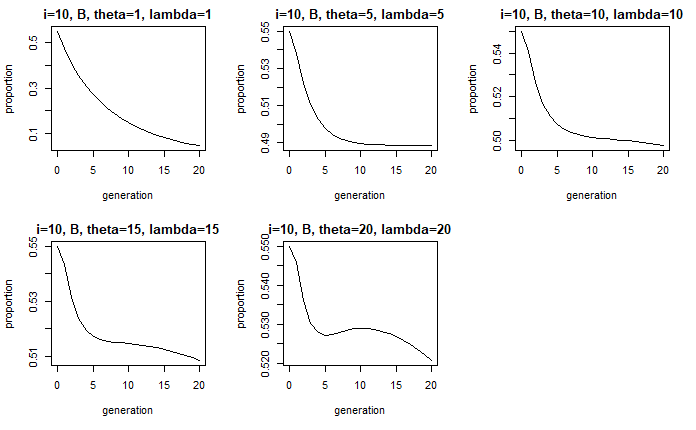
\includegraphics[scale = 0.6]{00003d.png}
\\
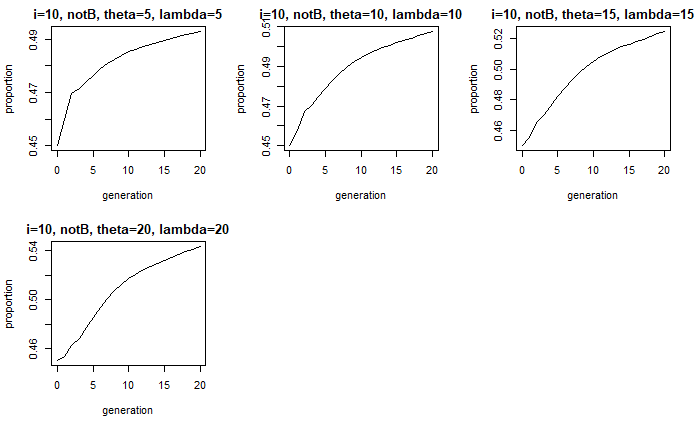
\includegraphics[scale = 0.6]{00006f.png}
\\
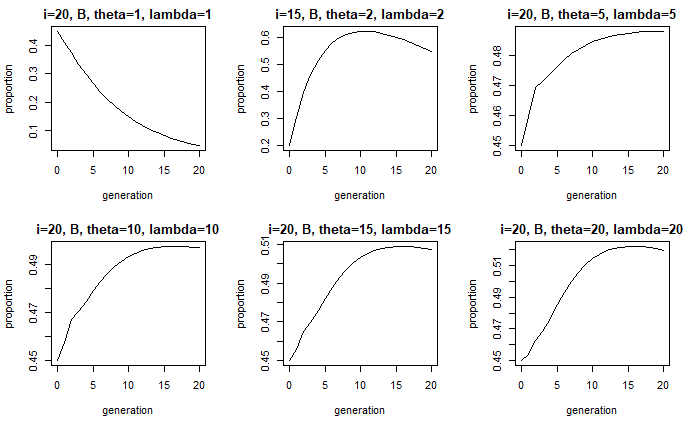
\includegraphics[scale = 0.6]{00002b.png}
\\
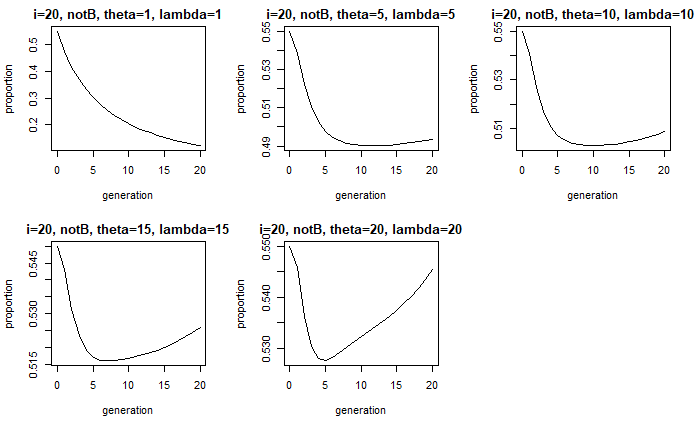
\includegraphics[scale = 0.6]{000017.png}
\\
And it is clear to see that, except for some special cases that the plots may look differently when $\lambda = \theta = 1$,  for other values the plots are all similar in terms of trend; thus, we say that $\lambda$ and $\theta$ values have no impact on the trend in most cases, with only influences on the time it takes to get to steady state. In details, when we focus on the sub-population group 10 with behavior B (when $i$ = 10), with value of $\theta$ and $\lambda$ increases the system becomes less stable and the time it takes to enter steady state increases; however, with large $i$ a completely different trend  can be observed: with $i$ = 20 the system is clearly getting more stable with increasing $\lambda$ and $\theta$. When it comes to behavior not B, the trends reverse entirely. This can be explained by the default setting of subgroups: groups from 1 to 10 are assumed to prefer behavior B, while the rest are assumed to prefer behavior not B. A conclusion can be drawn: if the behavior B is preferred originally in the sub-population group, then with increasing $\lambda$ and $\theta$ the stability of the system would increase; otherwise, the system would be less stable.
\\
\\
Plus, if we wish to study on any other parameters, it is the most safe choice to set $\lambda$ and $\theta$ to the average value 10 so that we can reduce the effect of $\lambda$ and $\theta$ as much as possible. Except that, there is another advantage of choosing  $\lambda$ = $\theta$ = 10: as what can be observed from the plots, in most cases, with the average delta-value and theta-value the system reaches its steady state very quickly; therefore, we can also reduce the effect of any possible non-steady-state values in the system by using $\lambda$ = $\theta$ = 10.
\\
\\
Another important parameter is $i$. Note that the initial values from group to group are different,  study on the change of trends with varying $i$ values would show the influences of initial values. We choose some of the specific groups with symbolic initial values and use plots to show its relevance:
\\
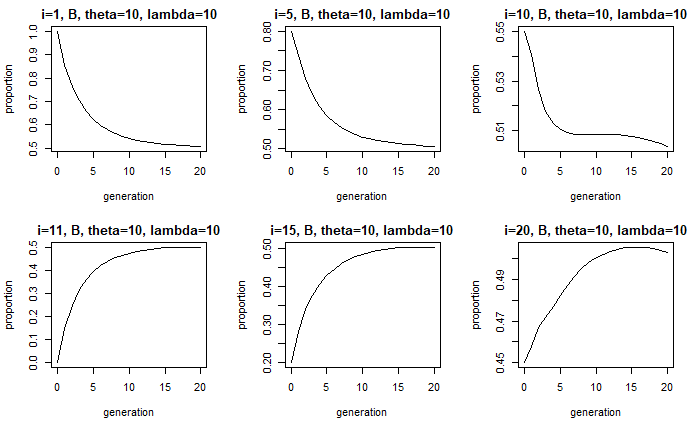
\includegraphics[scale = 0.6]{00002f.png}
\\
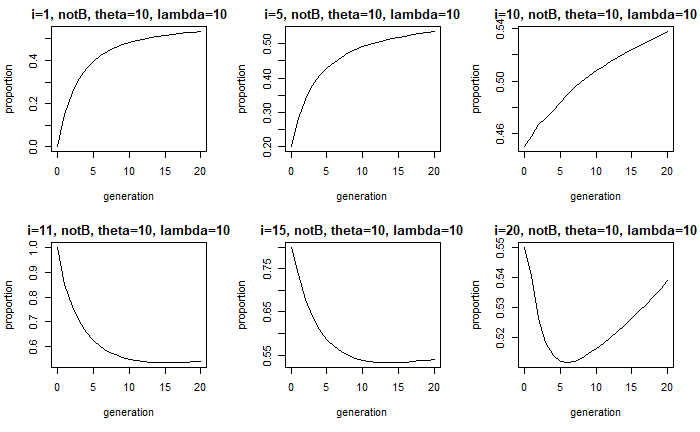
\includegraphics[scale = 0.6]{000047.png}
\\
Note that as $i$ values increase from 1 to 10 and from 11 to 20, the initial values for both behavior B and not B get close to 50\%; that is, the initial distribution of people who favor behavior B or not gets less extreme. By observing the plots, we can see that with changing initial values, the starting points in the plots are changed as well as the range of values; we can easily combine those plots with small range to those with large range. For instance, when $i$ = 20, the plot starts at proportion 0.45, and the plot can be seen as a part of the plot with $i$ = 11 but only with more details. Thus, we say that changing $i$ value has no effect.
\\
\\
Another important variable is the migration rate, $m$. In order to test the influence the parameter $m$ has on the system, we set any other variables as unchanged and use plots to show its impact. Let $\lambda = \theta = 10$ and we focus on the change of proportion of people who favor behavior B in subgroup 5. The plots are shown:
\\
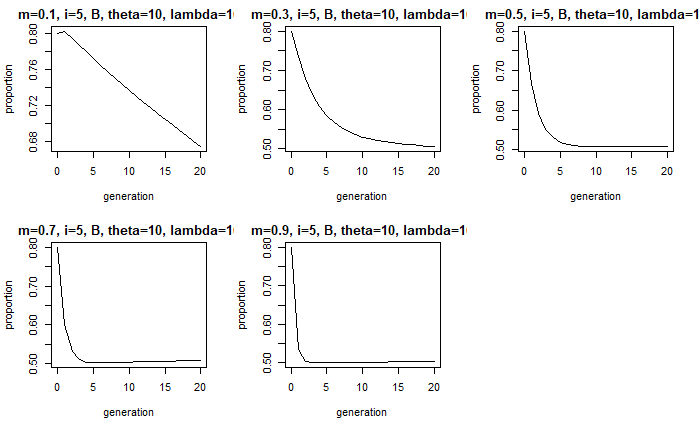
\includegraphics[scale = 0.6]{00002d1.png}
\\
Note that when $m$ value equals to 0.1, the plot is basically a straight line with negative increasing rate; as $m$ increases, the system starts to show a more and more stable steady state, ending at when the proportion of people who favor behavior B equals to around 50\%. Moreover, the time it takes to reach the steady state becomes shorter as $m$ increases: when $m = 0.3$ the system reaches steady state in around generation 20, while with $m = 0.9$ the system is already stable in the third generation. Thus, we say that with migration rate increases, the stability of the system increases.
\\
\section{Extending the Model -- Learning to Learn}
The model as designed by Boyd \& Richerson (1985) and Henrich \& Boyd (1998) assumes that individuals' temperament is entirely genetically determined and immutable throughout their lifetime. We were curious if relaxing this in some way, and treating $\lambda$ and $\theta$ more like $B$ would have any qualitative effect on the outcome of our simulation.
\\
\\
More precisely, we once again imagine that individuals experience environmental cues that may lead them to reject the behaviour that has been taught to them by their society. However, we imagine that such individuals will develop more cynical attitudes toward the very idea of learning socially, and come to more closely resemble those who have a genetic disposition favoring individual learning. Furthermore, this attitude, though not genetic, may be passed onto the individual's offspring through upbringing, and can therefore be modelled identically to a true change of genotype. This requires us to modify Equation (\ref{mod:2}).
\\
\\
In our extended model, after learning a behaviour $B$ from their society, individuals will, just as before, experience some environmental cue which has the potential to alter their choice of behaviour to $\lnot B$. However, we now assume that such an event will also have the effect of decrementing their $\lamba$-index such that they become less reliant on social learning generally. Furthermore, to balance out this effect and prevent ratcheting, we will also assume that when an individual experiences a sufficiently salient cue which confirms what they've been taught, they will become more trusting of socially transmitted knowledge, and hence experience an increase in their $\lambda$-index. The new equation is as follows:
\[
    u_{iB\lambda\theta}(t+.1)
        =
    \begin{cases}
        u_{iB\lambda\theta}(t+.0)
        -
        p_{(\lnot B) \lambda}
        \cdot 
        u_{iB\lambda\theta}(t+.0)
        +
        p_{B(\lambda-1)}
        \cdot 
        u_{Bi(\lambda-1)\theta}(t+.0)
        & \text{if $\lambda=\max \mathcal J$}
        \\
        \\
        u_{iB\lambda\theta}(t+.0)
        -
        p_{B\lambda}
        \cdot 
        u_{iB\lambda\theta}(t+.0)
        +
        p_{B(\lambda+1)}
        \cdot 
        u_{(\lnot B)i(\lambda+1)\theta}(t+.0)
        &
        \text{if $\lambda=\min \mathcal J$}
        \\
        \\
        u_{iB\lambda\theta}(t+.0)
        -
        [p_{B\lambda}+p_{(\lnot B)\lambda}]
        \cdot 
        u_{iB\lambda\theta}(t+.0)
        \\
        \hspace{1.75cm} +\ p_{B(\lambda+1)}
        \cdot 
        u_{(\lnot B)i(\lambda+1)\theta}(t+.0)
        +
        p_{B(\lambda-1)}
        \cdot 
        u_{Bi(\lambda-1)\theta}(t+.0)
        &
        \text{otherwise}
    \end{cases}
\]
Note that for the extended version of this model, we require that the set $\mathcal J$ be represented as a series of consecutive integers, such that for all $\lambda_1,\lambda_2\in\mathcal J$, $H_{\lambda_1}>H_{\lambda_2}$ if and only if $\lambda_1>\lambda_2$.


\section{Result for the Extended Model}

In the extension, the calculation of $u_{iB\lambda\delta}(t + 0.1)$ is modified in the way that extreme situations of when $j$ = max $J$ or min $J$ are considered as special cases; thus the way to calculate under these cases are different to the original one. In order to fully demonstrate the effect of doing so, again, we use plots to compare the results under same conditions generated by the two models:
\\
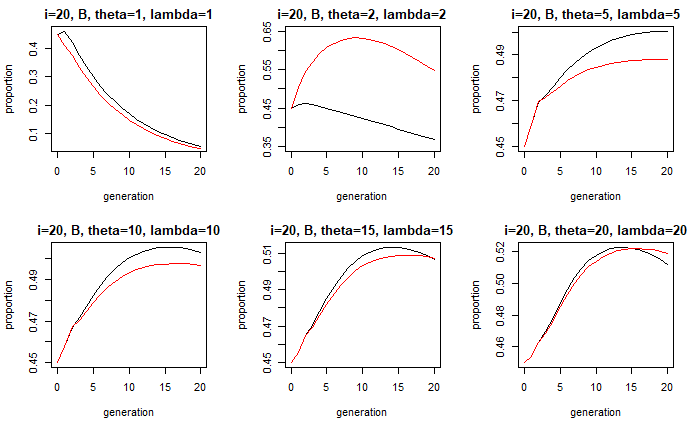
\includegraphics[scale = 0.6]{compare.png}
\\
where the black line represents the original model and the red line stands for the modified model.
\\
\\
As shown in the plots, generally the black line and red line have similar trends with minor differences; in the special case when $\theta = \lambda = 2$, though the two models give completely different results, it is clear that the red line fits the overall trend more than the black line does. Thus, we say that the extended model is basically an improve to the original model.
\\
\\
Since in this project our focus is the set of parameters that have possible impacts and what the influences are, we can simply ignore those minor differences since they do not change the overall trends. 

\section{Conclusion}
In all, two conclusions can be drawn from the results. For one, if the behavior B is preferred originally in the sub-population group, then with increasing $\lambda$ and $\theta$ the stability of the system that focuses on behavior B would increase; otherwise, the system would be less stable. This shows the effect of genotype \mbox{$(\lambda,\theta)$}: with values of $\lambda$ and $\theta$ increase, the effect of evolution, including learning, migration and selection, becomes stronger. With strong evolution effect, the initial condition becomes important. We can image a one dimensional axis with two opposite directions. If the group favors behavior B initially, then with high $\lambda$ and $\theta$ values the system focusing on behavior B would be stable, since the direction in the beginning fits the direction the evolution goes to; otherwise, the system focusing on behavior not B would be rather unstable, since the two directions do not fit.
\\
\\
Then, the stability of the system increases with migration rate increases. This is reasonable and fits our expectation: with high migration rate, the time it takes to process migration becomes shorter, which means that the process of the whole evolution would be faster. Therefore, with higher $m$, the system enters its steady state more quickly, and we say that the system is more stable.
\\
\\
In our extension, we did not account for the potential for for $\lambda$ and $\theta$ to themselves be inherited via conformist transmission, since it was found that doing so would require deep structural changes to the original model. This however would almost certainly be an interesting avenue for future study.
\\
\\
Even if the peculiarities of humans as a species can be entirely accounted for by our unique cultural inheritance patterns, it still leaves open the question of why humans were the only species to have evolved such patterns (Boyd \& Richerson, 1985). This fact remains an open question.


\newpage
\section{References}
Blackmore, S. (1999). \emph{The Meme Machine}. Oxford University Press. 
\\\\
Boyd, R., \& Richerson, P. J. (1985). \emph{Culture and the Evolutionary Process}. University of Chicago Press. 
\\\\
Brauer, F., Pauline, V. den D., Wu, J., \& S., A. L. J. (2008). \emph{Mathematical Epidemiology}. Springer. 
\\\\
Cavalli-Sforza, L. L., \& Feldman, M. W. (1983). \emph{Cultural versus genetic adaptation}. Proceedings of the National Academy of Sciences, 80(16), 4993–4996. \href{https://doi.org/10.1073/pnas.80.16.4993}{https://doi.org/10.1073/pnas.80.16.4993}
\\\\
Dawkins, R. (1982). \emph{The Extended Phenotype}. Oxford University Press. 
\\\\
Dawkins, R. (2006). \emph{In The Selfish Gene} (30th anniversary edition). Oxford University Press. 
\\\\
Henrich, J. (2014). \emph{The secret of our success: How culture is driving human evolution, domesticating our species, and making us smarter.} Princeton University Press. 
\\\\
Henrich, J. (2016, May 9). \emph{The Secret of Our Success}[Lecture recording]. Center for International Development at Harvard University. \href{https://www.youtube.com/watch?v=szTvEcsf578}{https://www.youtube.com/watch?v=szTvEcsf578}
\\\\
Henrich, J., \& Boyd, R. (1998). The evolution of conformist transmission and the emergence of between-group differences. \emph{Evolution and Human Behavior}, 19(4), 215–241. \href{https://doi.org/10.1016/s1090-5138(98)00018-x}{https://doi.org/10.1016/s1090-5138(98)00018-x}
\\\\
Herron, J. C., \& Freeman, S. (2014). \emph{Evolutionary Analysis}. Pearson. 
\\\\
Valen, M. V. (2020, January 5). \emph{The last word on ``The rhyme"}. Wild Snakes : Education and Discussion. Retrieved April 13, 2022, from \href{https://wsed.org/the-last-word-on-the-rhyme/}{https://wsed.org/the-last-word-on-the-rhyme/}
\end{document}
